\documentclass{article}
\usepackage[utf8]{inputenc}
\usepackage{amsmath}
\usepackage{amssymb}
\usepackage{graphicx}

\begin{document}
\section*{Structured matrix-vector product II}
We consider here another special matrix-vector product $\mathbf{x} = \mathbf{A}\mathbf{y}$ with 
\begin{equation*}
    \mathbf{A} = 
    \begin{bmatrix}
    a_{1} & &&& & a_{n} \\
     & a_{2} &&&  a_{n-1} &\\
     & &\ddots  &\text{\reflectbox{$\ddots$}}& & \\
     &&\text{\reflectbox{$\ddots$}} & \ddots& &  \\
     & a_{2} &&&  a_{n-1} &\\
     a_{1} &&&&& a_{n}
    \end{bmatrix}
\end{equation*}
which mathematically is defined as 
\begin{equation*}
    a_{ij} = 
    \begin{cases}
    a_{i} \quad &\text{if } i = j \\
    a_{j} &\text{if } i = n + 1 - j \\
    0 &\text{else.}
    \end{cases}
\end{equation*}
\subsection*{1-13.a} 
We are tasked with writing an efficient function that evaluates $\mathbf{y} = \mathbf{A}\mathbf{x}$ for the given matrix $\mathbf{A}$ and an input $\mathbf{x}$. We will first look at the structure of the matrix-vector product.
\begin{equation*}
\mathbf{A}\mathbf{x} = 
    \begin{bmatrix}
    a_{1} & &&& & a_{n} \\
     & a_{2} &&&  a_{n-1} &\\
     & &\ddots  &\text{\reflectbox{$\ddots$}}& & \\
     &&\text{\reflectbox{$\ddots$}} & \ddots& &  \\
     & a_{2} &&&  a_{n-1} &\\
     a_{1} &&&&& a_{n}
    \end{bmatrix} 
    \begin{bmatrix}
        x_{1} \\
        x_{2} \\
        \vdots \\
        \vdots \\
        x_{n-1} \\
        x_{n}
    \end{bmatrix} = 
    \begin{bmatrix}
        a_{1}x_{1} + a_{n}x_{n} \\
        a_{2}x_{2} + a_{n-1}x_{n-1} \\
        \vdots \\
        \vdots \\
        a_{2}x_{2} + a_{n-1}x_{n-1} \\
        a_{1}x_{1} + a_{n}x_{n}
    \end{bmatrix} = \mathbf{y}
\end{equation*}
We hence get
\begin{equation*}
    \left(\mathbf{y}\right)_{i} = a_{i}x_{i} + a_{n - i + 1}x_{n - i + 1} \quad \text{(Correct only for even $n$)}
\end{equation*}
Where we also can use that for $i > \left\lceil \frac{n}{2}\right\rvert$ we have $\left(\mathbf{y}\right)_{i} = \left(\mathbf{y}\right)_{n- i + 1}$. However we must be careful now, because if $n$ is odd the middle element is given by $\left(\mathbf{y}\right)_{\left\lceil \frac{n}{2}\right\rceil} = a_{\left\lceil \frac{n}{2}\right\rceil}x_{\left\lceil \frac{n}{2}\right\rceil}$. We must thus treat this case separately. 

\pagebreak

\noindent This gives us the following code.
\begin{figure}[!hbt]
    \centering
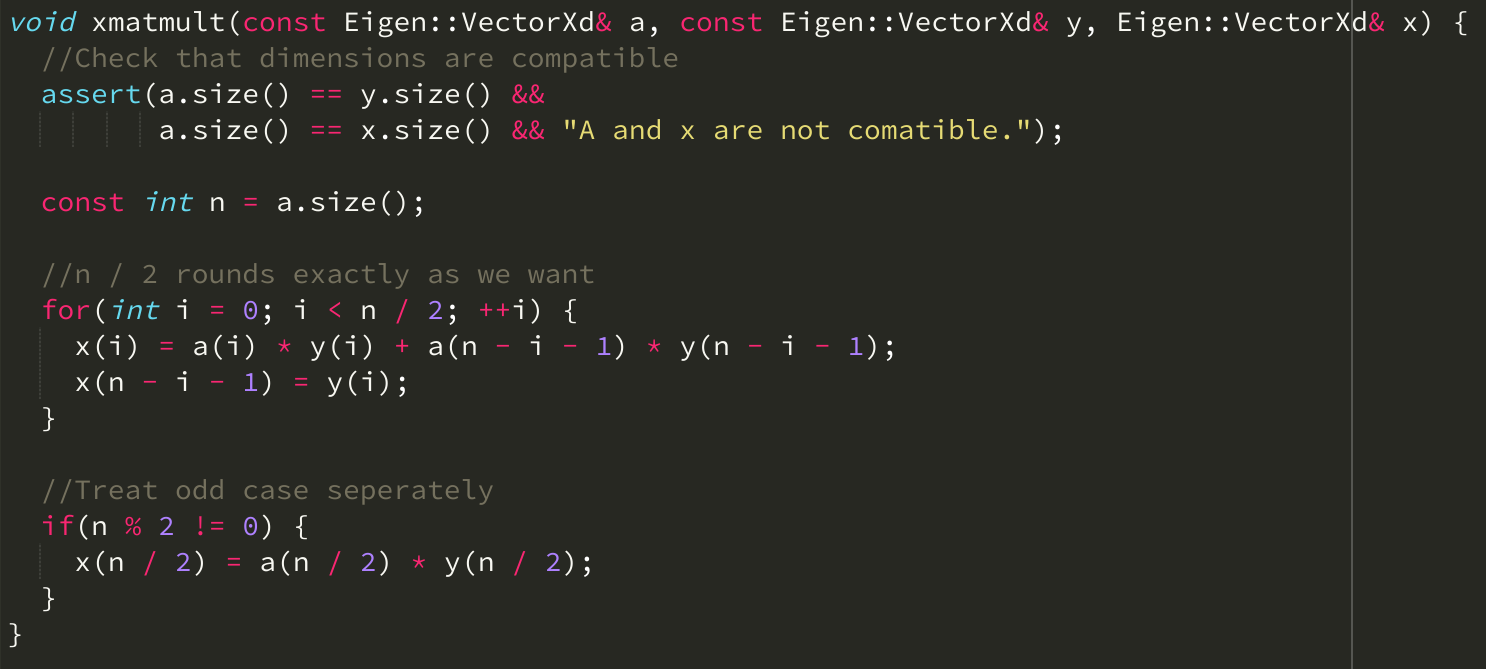
\includegraphics[width=1.0\linewidth]{1-13.a.png}
\end{figure}

\subsection*{1-13.b}
We are asked to state the asymptotic complexity with respect to the input size $n$. The loop does at most $\left\lceil \frac{n}{2}\right\rceil$ iterations, where each costs $\mathcal{O}\left(1\right)$ and hence we get $\mathcal{O}\left(n\right)$ overall, the cases where $n$ is odd adds only $\mathcal{O}\left(n\right)$ computational cost and hence overall we get a computational cost of $\mathcal{O}\left(n\right)$.
\subsection*{1-13.c}
(The tabulation was skipped as it is a reoccurring task that adds little to the learning process) The runtime for the conventional matrix-vector product will give us an $\mathcal{O}\left(n^{2}\right)$ asymptotic complexity.

\end{document}
